\section{Conceptos fundamentales en robótica de enjambre}

\subsection{Enjambre}
En la robótica, un enjambre es el conjunto de individuos que colaboran entre sí para lograr un objetivo. En la Figura \ref{fig:enjambre} se muestra un enjambre de robots.

\begin{figure}[H]
	\centering
	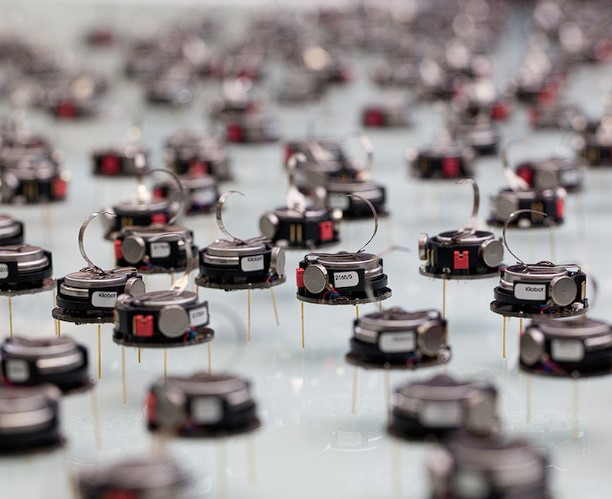
\includegraphics[width=0.6\textwidth]{enjambre.jpg}
	\caption{Ejemplo de enjambre de robots \cite{imgEnjambre}.}
	\label{fig:enjambre}
\end{figure}

\subsection{Agente}
Se le conoce como agente a un individuo que forma parte del enjambre. Este es capaz de realizar acciones simples para lograr un objetivo de forma colaborativa con los demás individuos. En la robótica de enjambre, los agentes son robots \cite{definiciones_robotica_enjambre}.

\subsection{Formaciones}
Es común que en la naturaleza se observen enjambres que forman patrones. Esto es gracias a que los individuos realizan movimientos coordinados para crear formaciones. En la robótica de enjambre sucede lo mismo, se tiene un conjunto de agentes que se organizan y coordinan sus movimientos para lograr objetivos. Estos pueden ser evadir obstáculos, mapear un entorno, llegar a un objetivo siguiendo una trayectoria, entre otros. Para lograr la coordinación de formaciones, se requiere aplicar un control que puede ser centralizado o descentralizado \cite{definiciones_robotica_enjambre}.

\subsection{Control centralizado y descentralizado}
En la robótica de enjambre, el control centralizado consiste en una red de comunicación donde una unidad central de procesamiento (CPU) tiene comunicación con cada agente para transmitir y recibir información. Asimismo, cada agente se comunica únicamente con el CPU.

El control descentralizado, también llamado control distribuido, es donde cada agente tiene comunicación con los demás para transmitir información. Este tipo de control requiere un protocolo de comunicación más robusto y complejo, sin necesidad de un CPU \cite{Control_centralizado_descentralizado}.

En la Figura \ref{fig:control_centralizado_descentralizado} se observa la diferencia entre ambos tipos de control.

\begin{figure}[H]
	\centering
	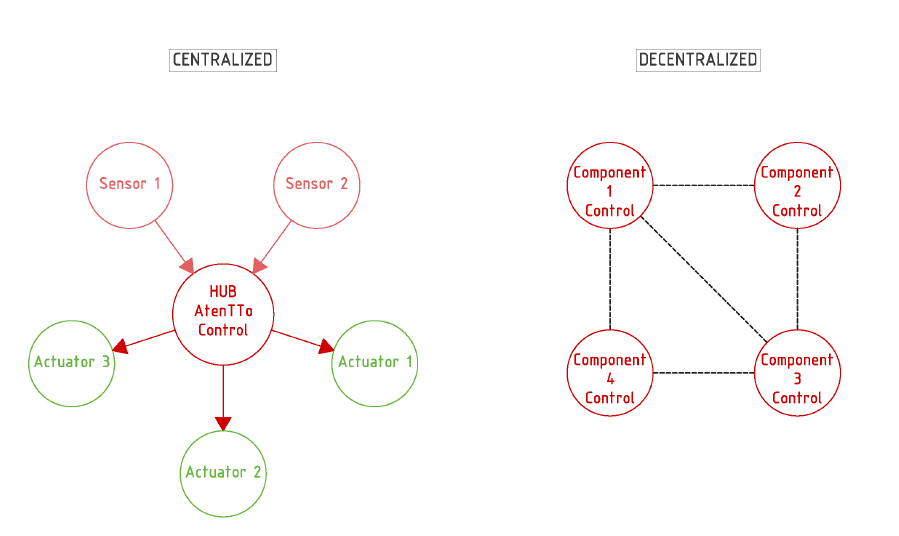
\includegraphics[width=1\textwidth]{control_centralizado_descentralizado.png}
	\caption{Ejemplo de un control centralizado y descentralizado \cite{Control_centralizado_descentralizado}.}
	\label{fig:control_centralizado_descentralizado}
\end{figure}


\section{Conceptos básicos en Teoría de grafos}

\subsection{Teoría de grafos}
La teoría de grafos es una rama de la matemática y ciencias de la computación que se dedica a estudiar los grafos \cite{teoria_de_grafos}. El grafo es un conjunto de vértices conectados por aristas tal como se observa en la Figura \ref{fig:teoria_de_grafos}. Esta teoría se utiliza en diversas aplicaciones como mapeo de entornos, generación de rutas, análisis de datos, telecomunicaciones, entre otras. En este trabajo de graduación, se utilizó la teoría de grafos para definir formaciones y la red de comunicación entre agentes.

\begin{figure}[H]
	\centering
	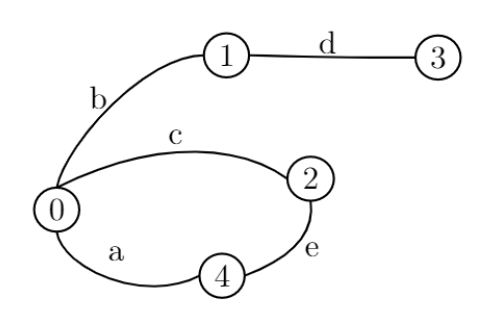
\includegraphics[width=0.5\textwidth]{grafo_matrices_andrea.png}
	\caption{Ejemplo de un grafo \cite{PenaAM_2019_tesis}.}
	\label{fig:teoria_de_grafos}
\end{figure}

\subsection{Vértices y aristas}
Los vértices, también llamados nodos, son los puntos donde se conectan las aristas de un grafo. El grado de un vértice será el número de aristas asociados a él \cite{teoria_de_grafos}. 

Las aristas, también llamadas arcos o enlaces, son las líneas que conectan un par de vértices y se clasifican en \cite{teoria_de_grafos}:

\begin{itemize}
	\item Lazo: Es una arista que tiene en sus extremos el mismo vértice. 
	\item Paralelas o múltiples: Es cuando dos o más aristas tienen en los extremos el mismo par de vértices.
\end{itemize}

\subsection{Tipos de grafos}
En un grafo, los vértices se puede conectar de distintas maneras según la aplicación que se requiera tal como se observa en la Figura \ref{fig:tipos_de_grafos}. Algunas de sus clasificaciones son \cite{tipos_de_grafos}:

\begin{itemize}
	\item Simple o anillo: Cada par de nodos se conecta por una sola arista.
	\item Multigrafo: En cada par de nodos puede haber más de un enlace.
	\item Árbol: Es un grafo que no tiene ciclos.
	\item Dirigidos o dígrafos: Las aristas entre los nodos tienen dirección.
	\item Estrella: Tiene un nodo central que conecta con los demás nodos.
	\item No conexos: Hay uno o más nodos que no conectan con el resto.
	\item Completo: Cada nodo está conectado con los demás.
	\item Regular: Todos los nodos tienen el mismo número de aristas.
	\item De celosía y mundo pequeño: Estos grafos se utilizan para entender el comportamiento y estructura de ciertos fenómenos en la naturaleza.
\end{itemize}

\begin{figure}[H]
	\centering
	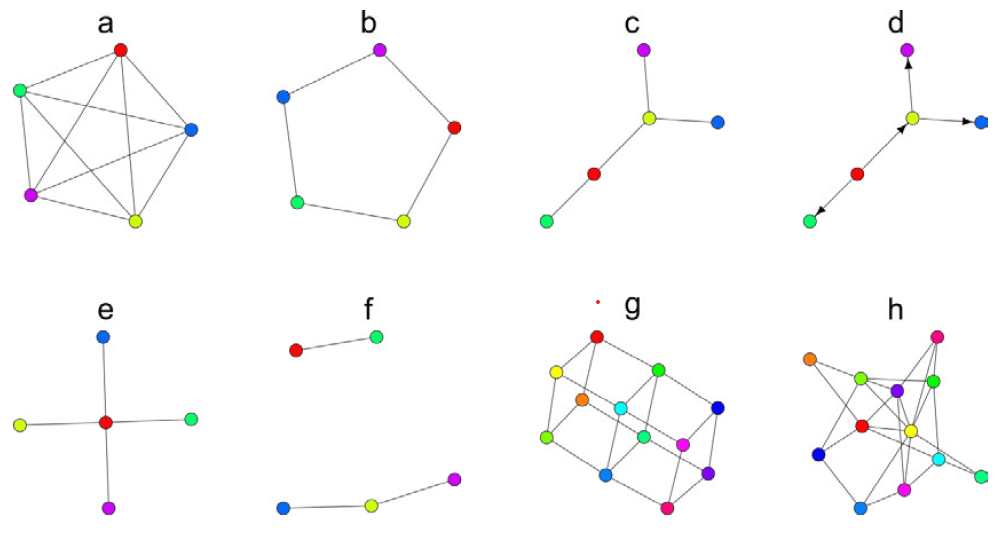
\includegraphics[width=1\textwidth]{tipos_de_grafos.png}
	\caption{Ejemplo de algunos tipos de grafos. a: completo, b: simple, c: árbol, d: dígrafo, e: estrella, f: no conexo, g: de celosía, h: de mundo pequeño \cite{tipos_de_grafos}.}
	\label{fig:tipos_de_grafos}
\end{figure}

\subsection{Matrices asociadas a un grafo}
La representación gráfica de un grafo es poco práctica para su análisis, por esto es mejor utilizar su representación matricial \cite{FrancoF_2016_trabajo_fin_de_grado}. A continuación, se mencionan algunas matrices útiles y su implementación para el grafo de la Figura \ref{fig:teoria_de_grafos}.


\begin{itemize}
	\item Matriz de incidencia (I): Se tiene una matriz de $v$ vértices por $e$ aristas. El elemento $a_{ve} = 1 $ si la arista conecta con el vértice, de lo contrario $a_{ve} = 0$
	
	\[
	I = 
	\left[\begin{array}{ccccc}
		1 & 1 & 1 & 0 & 0 \\
		0 & 1 & 0 & 1 & 0 \\
		0 & 0 & 1 & 0 & 1 \\
		0 & 0 & 0 & 1 & 0 \\
		1 & 0 & 0 & 0 & 1 \\
	\end{array} \right]
	\]
	
	\item Matriz de adyacencia (A): El grafo se representa con una matriz cuadrada de tamaño $v \times v$. Si hay una arista entre el vértice $v_1$ y $v_2$ , el elemento $a_{v_1 v_2} = 1$.
	
	\[
	A = 
	\left[\begin{array}{ccccc}
		1 & 1 & 0 & 0 & 0 \\
		0 & 0 & 1 & 1 & 0 \\
		0 & 0 & 0 & 1 & 0 \\
		0 & 0 & 0 & 0 & 0 \\
		0 & 0 & 0 & 0 & 0 \\
	\end{array} \right]
	\]
	
	\item Matriz de grados (D): Se tiene una matriz diagonal de tamaño $v \times v$ que contiene los grados de cada vértice. 
	
	\[
	D = 
	\left[\begin{array}{ccccc}
		3 & 0 & 0 & 0 & 0 \\
		0 & 2 & 0 & 0 & 0 \\
		0 & 0 & 2 & 0 & 0 \\
		0 & 0 & 0 & 1 & 0 \\
		0 & 0 & 0 & 0 & 2 \\
	\end{array} \right]
	\]
	
	\item Matriz laplaciana (L): Esta matriz es resultado de operar otras matrices asociadas al grafo. Para grafos no dirigidos, esta se calcula como $L = D - A$. Para grafos dirigidos se calcula como $L = I I^T$.
	
	\[
	l = 
	\left[\begin{array}{ccccc}
		3 & -1 & -1 & 0 & -1 \\
		-1 & 2 & 0 & -1 & 0 \\
		-1 & 0 & 2 & 0 & -1 \\
		0 & -1 & 0 & 1 & 0 \\
		-1 & 0 & -1 & 0 & 2 \\
	\end{array} \right]
	\]
	
	\item Matriz de rigidez (K): Esta matriz surge de qué tanto es posible deformar el grafo sin doblar ni modificar la longitud de las aristas \cite{matrices_asociadas_grafos}. A continuación se muestra la matriz de adyacencia totalmente rígida.
	
	\[
	A = 
	\left[\begin{array}{ccccc}
		1 & 1 & 0 & 0 & 0 \\
		0 & 0 & 1 & 1 & 0 \\
		0 & 0 & 0 & 1 & 0 \\
		0 & 0 & 0 & 0 & 0 \\
		0 & 0 & 0 & 0 & 0 \\
	\end{array} \right]
	\]
	
	Esta corresponde a la matriz de adyacencia del grafo completo.
	
\end{itemize}


\section{Control de la formación}
Para resolver el problema de control de formaciones se utilizan dos grafos asociados. El primero es el grafo de formación. Este es un grafo no dirigido que contiene la configuración deseada. Además, se utiliza un grafo ponderado donde las longitudes de las aristas representan la distancia entre los agentes. El segundo grafo es el que representa la red de comunicación entre agentes. Este es un grafo dirigido donde las aristas están definidas por la dinámica de lazo cerrado del sistema multi-agente \cite{PenaAM_2019_tesis}. 

\subsection{Grafo de formación}
Para definir un grafo de formación se debe entender el concepto de rigidez. Una estructura es rígida cuando todas las distancias entre los vértices están definidas y se mantienen constantes. Para evaluar la rigidez de un grafo se debe cumplir $e = 2v - 3$, donde $v$ es el número de vértices y $e$ el número de aristas. Si un grafo tiene menos aristas que vértices, este ya no se considera rígido \cite{KrickL_2007_tesis}.

Con esto, se introduce el término de un grafo mínimamente rígido. Para que un grafo se considere mínimamente rígido, debe tener un estado donde si se elimina cualquier arista, el grafo deja de ser rígido.

La ventaja de trabajar con grafos mínimamente rígidos es que no tienen restricciones innecesarias a la hora de mantener la formación.

\begin{figure}[H]
	\centering
	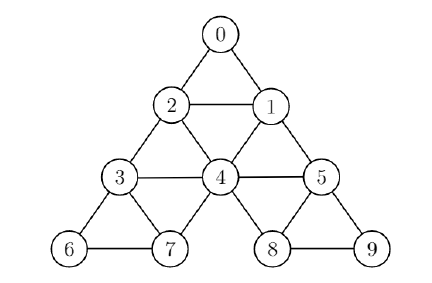
\includegraphics[width=0.4\textwidth]{grafo_formacion_triangular.png}
	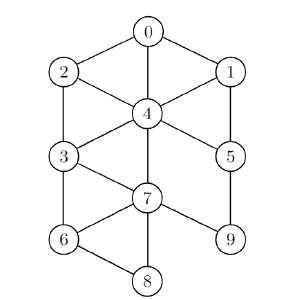
\includegraphics[width=0.4\textwidth]{grafo_formacion_hexagonal.png}
	\caption{Grafos de formación en triángulo y hexágono \cite{PenaAM_2019_tesis}.}
	\label{fig:grafos_formación}
\end{figure}

\subsection{Construcción de un grafo mínimamente rígido}
El método de Henneberg es utilizado para construir grafos mínimamente rígidos donde cada vértice mantiene dos grados de libertad \cite{KrickL_2007_tesis}. Los pasos para realizar el método son:

\begin{enumerate}
	\item Numerar todos los vértices.
	\item Agregar una arista entre el vértice 1 y el vértice 2.
	\item Agregan los demás vértices a la estructura utilizando dos aristas.
	\item Verificar que se cumple la condición de $e = \frac{v^2-v}{2}$
\end{enumerate}


\subsection{Grafo para la red de comunicación}
La comunicación entre agentes se representa por un grafo de comunicación. Este es un dígrafo que indica cuáles agentes tienen comunicación entre ellos y hacia qué dirección se comunican \cite{grafos_en_redes_multiagente}. A continuación se muestran tres tipos de redes.

\begin{itemize}
	\item Red estática: Las aristas se mantienen invariantes en el tiempo.
	\item Red dinámica o dependiente del estado: Las aristas son variantes en el tiempo y pueden desaparecer o aparecer según el estado de la red de agentes.
	\item Red aleatoria: La existencia de una arista se da mediante una distribución de probabilidad.
\end{itemize}

\section{Teoría de control}
En la robótica, se utilizan sistemas de control que integran varios subsistemas y procesos para estabilizar una respuesta inestable. Esto se logra mediante la implementación de un controlador que manipula las entradas del sistema para obtener la salida deseada \cite{control_lazo_cerrado}. En la Figura \ref{fig:lazo_cerrado_control} se muestra el sistema de control más utilizado.

\begin{figure}[H]
	\centering
	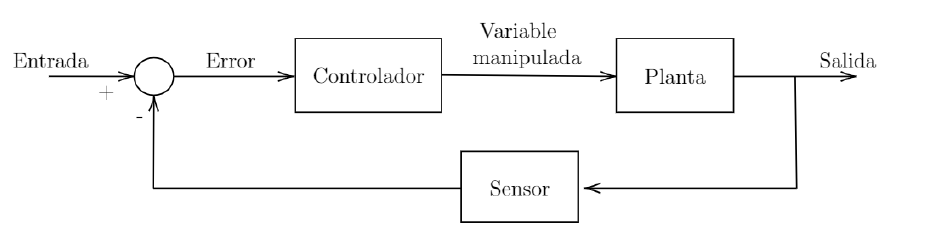
\includegraphics[width=0.8\textwidth]{lazo_cerrado_control.png}
	\caption{Sistema de control en lazo cerrado \cite{control_lazo_cerrado}.}
	\label{fig:lazo_cerrado_control}
\end{figure}

\subsection{Control de formación}
Para realizar el control de formaciones se requieren dos niveles de control, uno superior y otro inferior. El control de capa superior maneja el comportamiento de los agentes y sus posiciones. El control de capa inferior controla la velocidad de las ruedas en cada agente \cite{PenaAM_2019_tesis}.

\section{Cinemática de robots diferenciales con ruedas}
Para la implementación física en la robótica de enjambre se requiere un modelo de movimiento que contemple las dimensiones y características físicas del robot como se observa en la Figura \ref{fig:modelo_uniciclo}. Para esto se tienen las ecuaciones (\ref{eq:velocidad_lineal_uniciclo}) y (\ref{eq:velocidad_angular_uniciclo}). Donde $\ell$ es la distancia del motor hasta su centro, $\varphi$ es el ángulo de orientación del uniciclo dentro del plano $XY$, $v$ es la velocidad lineal del robot, $w$ es la velocidad angular de las ruedas y $r$ es el radio de las ruedas \cite{ZeaM_modelo_uniciclo}.

\begin{equation}
	v = \frac{r(\dot{\varphi}_R + \dot{\varphi}_L)}{2}
	\label{eq:velocidad_lineal_uniciclo}
\end{equation}

\begin{equation}
	w = \frac{r(\dot{\varphi}_R + \dot{\varphi}_L)}{2\ell}
	\label{eq:velocidad_angular_uniciclo}
\end{equation}

\begin{figure}[H]
	\centering
	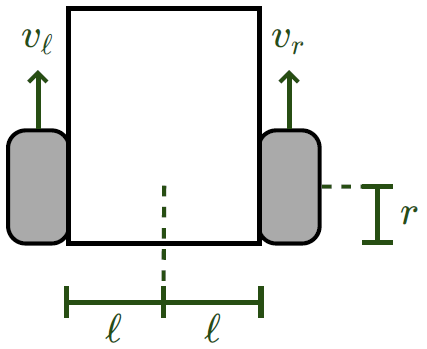
\includegraphics[width=0.5\textwidth]{modelo_uniciclo.png}
	\caption{Modelo de uniciclo \cite{ZeaM_modelo_uniciclo}.}
	\label{fig:modelo_uniciclo}
\end{figure}

Adicional a esto, se puede calcular la velocidad controlada de la rueda derecha y la rueda izquierda con las ecuaciones (\ref{eq:velocidad_controlada_derecha}) y (\ref{eq:velocidad_controlada_izquierda}), respectivamente.

\begin{equation}
	\dot{\varphi}_{R,crtl} = \frac{v_{ctrl} + \ell w_{crtl}}{r}
	\label{eq:velocidad_controlada_derecha}
\end{equation}

\begin{equation}
	\dot{\varphi}_{L,crtl} = \frac{v_{ctrl} - \ell w_{crtl}}{r}
	\label{eq:velocidad_controlada_izquierda}
\end{equation}

\section{Otras ecuaciones matemáticas relevantes}
Para mantener una correcta formación y distribución del enjambre, se necesitan herramientas como la ecuación de consenso y la función de tensión.

\subsection{Ecuación de consenso}
La ecuación \ref{eq:consenso} se utiliza para mantener la formación de los agentes en la posición asignada. Esta toma en cuenta el centro de masa de la formación y calcula la velocidad de cada agente para mantener la forma del grafo \cite{PenaAM_2019_tesis}.

\begin{equation}
	v_i(t) = \sum_{j \in N(i)} (x_j(t) - x_i(t)), i = 1, 2, ..., n
	\label{eq:consenso}
\end{equation}

Donde $N(i)$ es el conjunto de unidades adyacentes de la unidad $i$ en la red multi-agente.

Luego de añadir los pesos, se obtiene la ecuación \ref{eq:consenso2}:

\begin{equation}
	\frac{\partial \varepsilon_{i,j}}{\partial x_i} = w_{i,j}(\Vert x_i - x_j \Vert)(x_i - x_j)
	\label{eq:consenso2}
\end{equation}

Donde de puede despejar el peso $w_{i,j}$.

\subsection{Funciones racionales para hallar la tensión}
Para modificar la ecuación de consenso es necesario hallar la tensión utilizando funciones racionales que toman en cuenta las distancias deseadas y las distancias restringidas \cite{PenaAM_2019_tesis}.

\begin{itemize}
	\item Modelo 1: Combinación aditiva del control de formación y evasión de obstáculos.
	\begin{equation}
		\epsilon_{ij} = \frac{1}{2}(\Vert x_i - x_j \Vert - d_{ij})^2 + \frac{\Vert x_i - x_j \Vert^2}{\Vert x_i - x_j \Vert - r}
		\label{eq:ConsensoModelo1}
	\end{equation}
	Donde, $d_{ij}$ es la distancia entre los agentes $i$ y $j$, y $r$ es el radio de los agentes.
	
	\item Modelo 2: Combinación de control de formación, evasión de obstáculos y mantenimiento de la conectividad.
	\begin{equation}
		\epsilon_{ij} = \frac{(\Vert x_i - x_j \Vert - d_{ij})^2}{(\Vert x_i - x_j \Vert - r)(\Vert x_i - x_j \Vert - R)}
		\label{eq:ConsensoModelo2}
	\end{equation}
	Donde, $R$ es la distancia máxima que se pueden alejar los agentes sin salirse del rango del radar de los otros.
	
	\item Modelo 3: Combinación de control de formación y evasión de obstáculos.
	\begin{equation}
		\epsilon_{ij} = \frac{2(\Vert x_i - x_j \Vert - d_{ij})^2}{\Vert x_i - x_j \Vert - r}
		\label{eq:ConsensoModelo3}
	\end{equation}
	
	\item Modelo 4: Modelo dinámico con control de formación y evasión de obstáculos.\par
	
	Se utiliza un modelo dinámico que al inicio, cuando los agentes comienzan en posiciones aleatorias, se utiliza únicamente el control para evitar colisiones. Luego, cuando los agentes están lo suficientemente cerca sin chocarse, se cambia al modelo de la ecuación \ref{eq:ConsensoModelo3} que toma en cuenta el control de la formación 
	
	\item Modelo 5: Modelo dinámico con control de formación usando coseno hiperbólico y evasión de obstáculos.
	\begin{equation}
		\epsilon_{ij} = 0.01\cosh{(1.8 \Vert x_i - x_j \Vert - 8.4)}
		\label{eq:ConsensoModelo5}
	\end{equation}
	Se utilizó el coseno hiperbólico ya que es una función ``plana'' que permite que el control de formación sea el que decida dónde deben posicionarse los agentes en caso de tener un mínimo erróneo en una distancia de 0.
	
	\item Modelo 6: Modelo dinámico con control de formación usando coseno hiperbólico y evasión de obstáculos incluyendo límites de velocidad.\par
	Esta modificación no afecta directamente a la ecuación. Se realiza después de esta y consiste en incluir un límite de velocidad al modelo de la ecuación \ref{eq:ConsensoModelo5}. Por lo tanto, si la velocidad obtenida con el modelo es mayor al límite establecido, solo se tomará en cuenta la dirección.
	
\end{itemize}

\section{Herramientas de software}
Para realizar los cálculos, el control y las pruebas con los agentes robóticos, se necesita utilizar software especializado como los siguientes:

\subsection{Matlab}
Matlab es una plataforma de programación desarrollada por MathWorks con su propio lenguaje especializado para aplicaciones de ingeniería, análisis de datos, generación de algoritmos, entre otras \cite{matlab}.

Para el presente trabajo, se utiliza Matlab como la fuente de procesamiento de datos y generación de trayectorias para el algoritmo de sincronización y control de formaciones.

\subsection{Entorno de simulación Webots}
Webots es un software de código abierto creado por Cyberbotics \cite{webots}. Esta plataforma se centra en la simulación de escenarios que permiten replicar situaciones reales con distintos tipos de robots y objetos tal como se muestra en la Figura \ref{fig:webots}. Varios de los modelos disponibles en Webots están calibrados para comportarse como el modelo real y el usuario puede modificar los parámetros para garantizar una simulación realista.

Webots también cuenta con la implementación de controladores en lenguajes como C, C$++$, Matlab, Python, Java, ROS, o con API.

\begin{figure}[H]
	\centering
	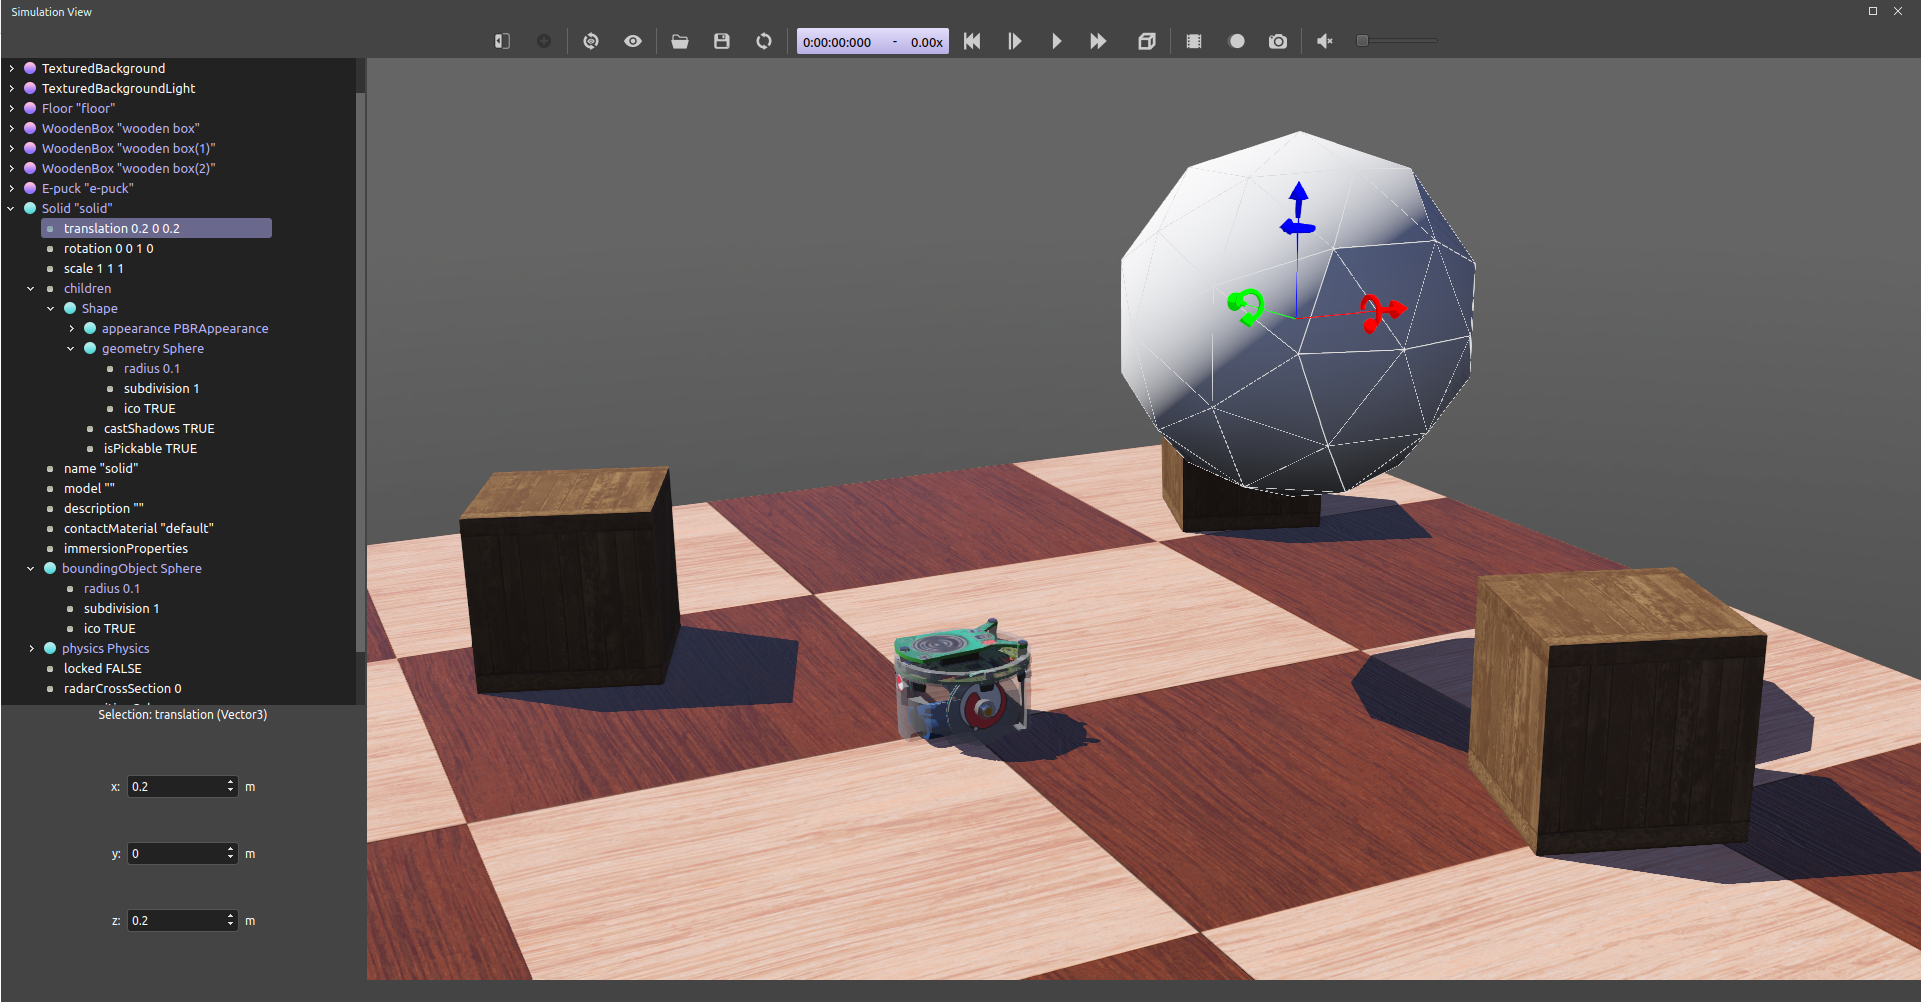
\includegraphics[width=0.8\textwidth]{webots.png}
	\caption{Entorno de simulación en Webots \cite{webots}.}
	\label{fig:webots}
\end{figure}

\subsection{Paralelismo computacional}
Al momento de trabajar con algoritmos y problemas complejos, se requiere utilizar métodos de optimización de software para agilizar el procesamiento de cálculos y la ejecución de tareas. 
Para esto, se utilizan herramientas como el paralelismo computacional. Consiste en dividir las tareas y asignarlas a cada núcleo del procesador para ejecutarlas simultáneamente \cite{libro_paralelismo}. Esto reduce considerablemente el tiempo de procesamiento. Además es importante considerar las dependencias entre las tareas como:

\begin{itemize}
	\item Dependencia de control de secuencia: Es el orden secuencial clásico de los algoritmos secuenciales.
	\item Dependencia de comunicación: Es cuando una tarea depende de la información que envíe otra tarea.
\end{itemize}

En la Figura \ref{fig:paralelismo_dependencia_tareas} se observa un ejemplo donde puede existir tiempos muertos ya que la tarea 3 depende de la información enviada por la tarea 1 y la tarea 4 depende de la información enviada por la tarea 3.
\begin{figure}[H]
	\centering
	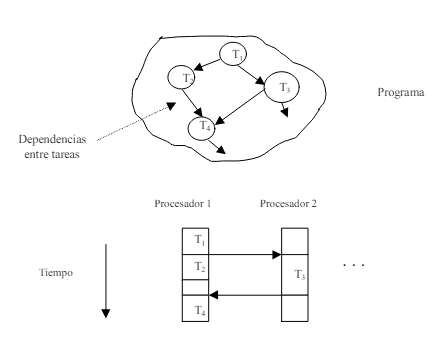
\includegraphics[width=0.6\textwidth]{paralelismo_dependencia_tareas.png}
	\caption{Ejemplo de dependencia de tareas \cite{libro_paralelismo}.}
	\label{fig:paralelismo_dependencia_tareas}
\end{figure}

\section{Ecosistema Robotat}
El Robotat es una plataforma que cuenta con herramientas y sistemas de captura de movimiento útiles para experimentar con la robótica de enjambre. A continuación se describen las herramientas más importantes.

\subsection{Mesa de pruebas}
Es una plataforma de acero y plycem con un espacio útil de $5 \times 5 \times 3$ m, capaz de soportar cargas puntuales de hasta dos toneladas. 

\subsection{Sistema de captura de movimiento OptiTrack}
Es un sistema de captura de movimiento que consta de 6 cámaras OptiTrack Prime$^x$ 41 al rededor de la mesa de pruebas. Estas son cámaras de alta precisión y baja latencia que permiten realizar experimentos en tiempo real. En la Figura \ref{fig:OptiTrack_primex41} se muestra el modelo disponible en la Universidad del Valle de Guatemala que tiene las siguientes características \cite{primex41}:

\begin{itemize}
	\item Resolución de 4.1 mega píxeles (MP).
	\item Precisión de $\pm$ 0.10 mm.
	\item Errores rotacionales menores a 0.5 grados.
	\item Lentes de 12 mm.
	\item Tasa de refresco nativa de 180 FPS con un un máximo de hasta 250 FPS.
	\item Distancia de captura de hasta 100 pies desde la cámara al marcador.
	\item Rango de captura de hasta 290,000 pies cúbicos por cámara para marcadores pasivos
	\item Rango de captura de hasta 1,000,000 pies cúbicos por cámara para marcadores activos.
\end{itemize}

\begin{figure}[H]
	\centering
	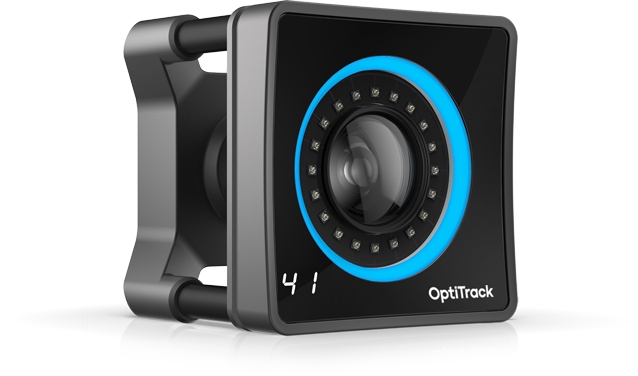
\includegraphics[width=0.5\textwidth]{primex41.png}
	\caption{Cámara de captura de movimiento Prime$^x$ 41 de OptiTrack \cite{primex41}.}
	\label{fig:OptiTrack_primex41}
\end{figure}

\subsection{Comunicación del Robotat}
La plataforma del Robotat utiliza un protocolo de comunicación TCP para transmitir la información de las cámaras OptiTrack al servidor principal del laboratorio. Este servidor de Python envía los datos a través de Wi-Fi en una red local. A esta red local, se puede acceder con una computadora para extraer la información que se necesite, además las plataformas robóticas también se pueden conectar a la red local para recibir instrucciones.

\section{Hardware}
Para poner a prueba el algoritmo de sincronización y control de formaciones en un ambiente físico, se necesita de una plataforma robótica móvil que en este proyecto será el Pololu 3pi+. 

\subsection{Plataforma móvil Pololu 3pi+ modificado}
La plataforma móvil a utilizar es una modificación basada en el Pololu 3pi+ 32U4 OLED Robot \cite{pololu3pi+}. Tiene un diámetro de 97 mm y altura de 36 mm, además, cuenta con lo siguiente:
\begin{itemize}
	\item Procesador ATmega34U4 MCU @ 16 MHz.
	\item Sensores de línea y de choque frontales.
	\item Encoders de doble cuadratura para control de posición y velocidad en lazo cerrado.
	\item IMU (acelerómetro de 3 ejes, magnetómetro y giroscopio).
	\item Pantalla OLED integrada.
\end{itemize}

\begin{figure}[H]
	\centering
	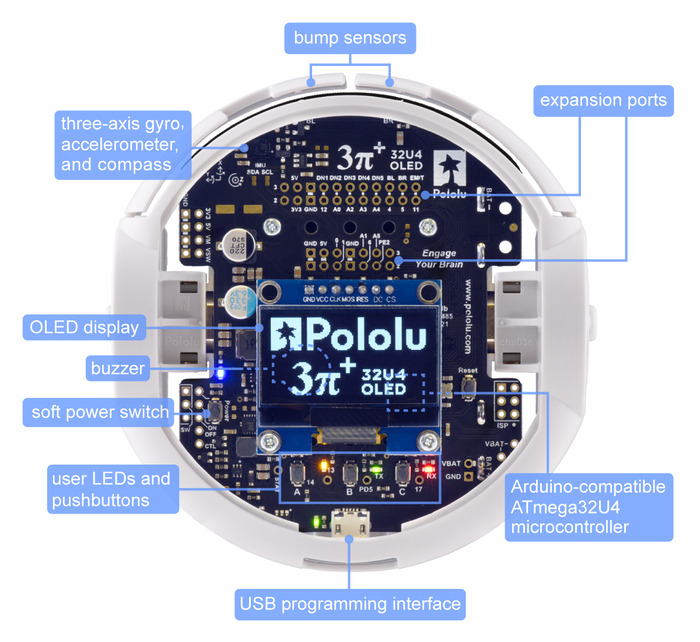
\includegraphics[width=0.45\textwidth]{pololu_sensores1.jpg} 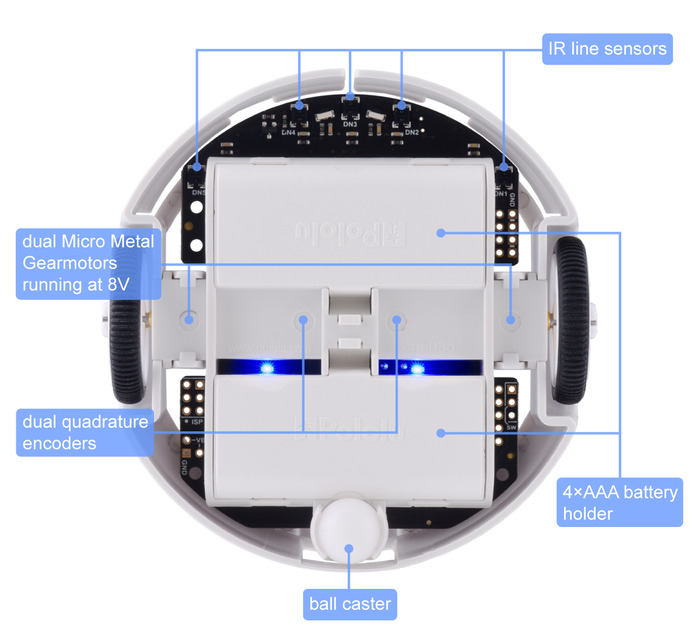
\includegraphics[width=0.45\textwidth]{pololu_sensores2.jpg}
	\caption{Sensores y componentes del Pololu 3pi+ 32U4 OLED Robot \cite{pololu3pi+}.}
	\label{fig:pololu_sensores}
\end{figure}

A esta plataforma móvil se le adaptó un ESP32 ya que el microcontrolador original tiene poca capacidad de procesamiento. Esto permitió tener control de capa superior e inferior, además de incorporar una red de comunicación WiFi con el Robotat para controlar los agentes.








